\section{Design}
\label{sec:design}
\system{} is a system that provides oblivious content distribution and is 
comprised of the following components: clients, exit proxies, CDNs, and origin 
servers.  Clients are the internet users who use the system to access content 
stored on CDN cache nodes; exit proxies are proxies that obfuscate the requests 
and responses retrieved from the CDNs; and the origin servers are the content 
publishers who are customers of the CDNs.  Figure \ref{fig:ocd_overview} shows how
these components interact in the system.  This section describes the decisions 
made in the design of \system{}, and what functionality each decision provides.  
We separate design decisions into two parts: 1) setup decisions and 2) request/
response decisions.  We also highlight some additional options that the design of 
\system{} allows.

\begin{figure}[t!]
\centering
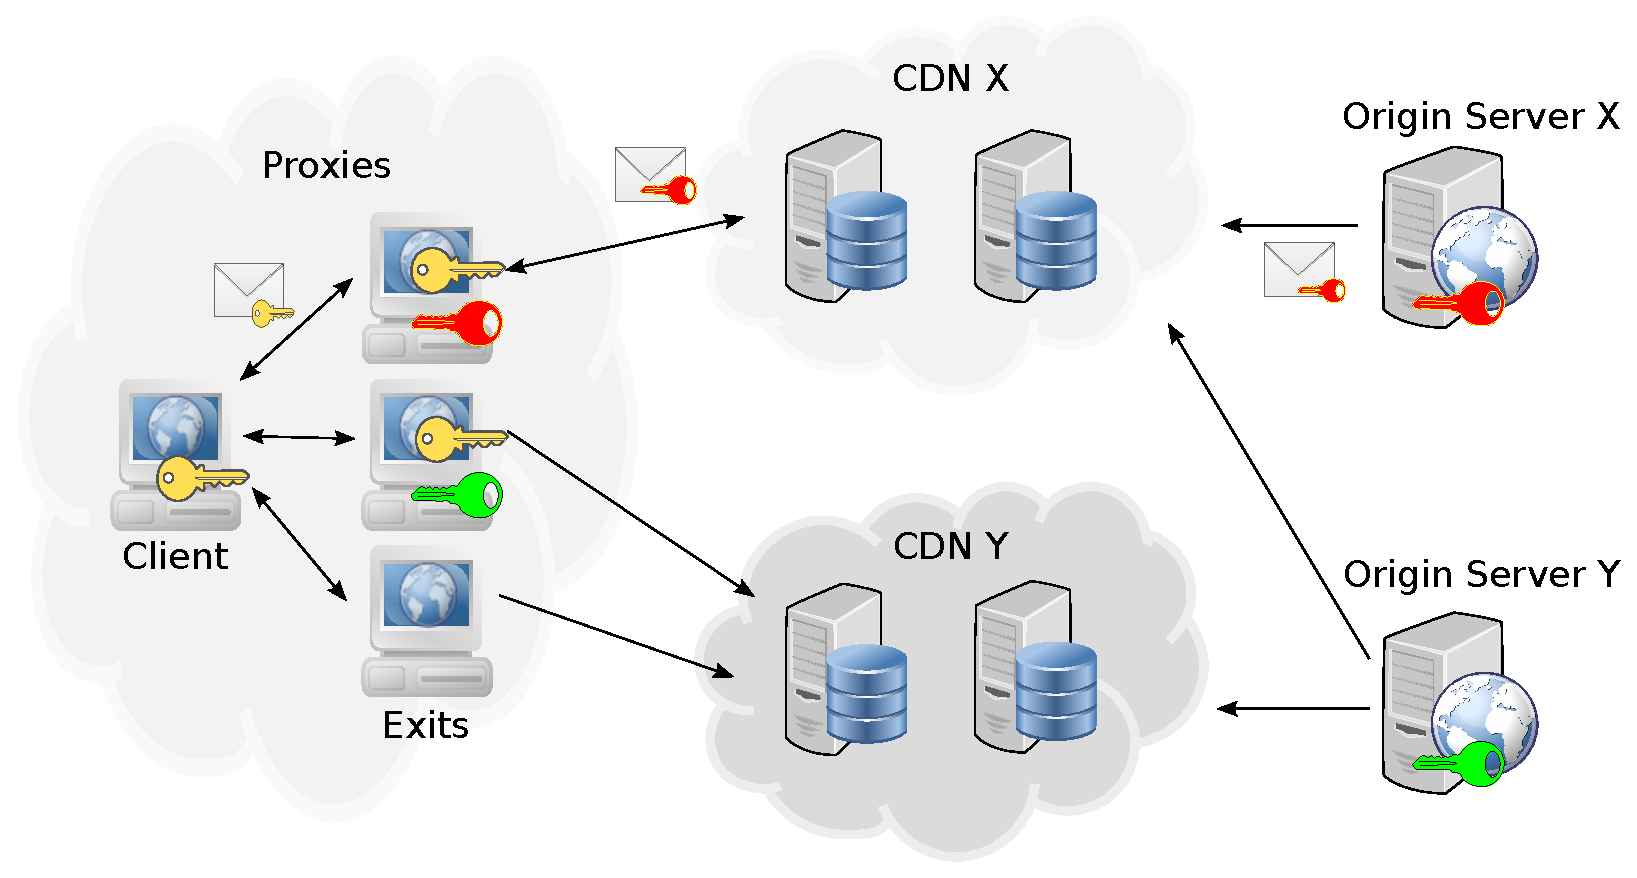
\includegraphics[width=.5\textwidth]{ocdn_overview_new2}
\caption{The relationships between clients, exit proxies, CDNs, and origin servers in 
\system{}.}
\label{fig:ocd_overview}
\end{figure}

\subsection{\system{} Setup}
We start by discussing how the system components communicate and authenticate 
one another; these design decisions are outline in Table \ref{tab:setup}.  Here
we introduce shared keys between origin servers and exit proxies, how these keys are 
stored, how the exit proxies authenticate themselves to origin servers, and how these 
keys are distributed.

\begin{table*}[t!]
\centering
\begin{tabular}{| l | l |} 
\hline
 Design Decision & Functionality Provided \\
\hline \hline
 Shared Keys & {} \\
\hline
 Consistent Hashing & {} \\
\hline
 Self-Certifying Identifiers & {} \\
\hline
 DNS for Key Sharing & {} \\
\hline
\end{tabular}
\caption{The design decisions associated with the setup and logistical aspects of \system{}, and what these decisions provide.}
\label{tab:setup}
\end{table*}

\paragraph{Shared Keys} 
To prevent an adversary from learning information, the CDN must not have the knowledge of what 
content it is caching.  Therefore, the content {\it and} the associated URL must be obfuscated 
before they enter the CDN.  The content can be obfuscated by encrypting it with a key that is not 
known to the CDN.  Because this must be done prior to any caching, the content publisher must 
generate a shared key $k$ to encrypt the content with. Encrypting the content alone does not 
hide much from the CDN; the content identifier, or URL, must also be obfuscated, otherwise the 
CDN can still reveal information about which clients accessed which URLs (which is indicative 
of the content).  In obfuscating the URL, the result should be a fixed, and relatively small size; 
these requirements are to preserve storage space and to prevent the adversary from guessing the 
URL based on the length of the obfuscated URL.  Unfortunately, using a simple hash allows an 
attacker to guess what the content identifier is by hashing his guesses and comparing with 
the hashes stored in the CDNs caches.  Therefore, the content publisher incorporates the use 
of the shared key $k$ into the hash of the URL by using a hash-based message authentication code 
(HMAC).  Additionally, if the domain supports HTTPS requests, then the content publisher must 
also encrypt the associated certificate with the same key $k$.

Then the encrypted content and HMAC are sent to the CDN\footnote{Most CDNs allow the publisher to 
decide on a push or pull model, but this makes no difference in our system design.} and stored in 
its caches.  The content publisher then shares the key $k$ with an exit proxy.  This allows the 
exit proxy to request encrypted content on behalf of clients by computing the HMAC on the URL.  

\paragraph{Consistent Hashing}
Each exit proxy stores a mapping of URLs to their associated shared key $k$; for example, if 
an origin server has shared key $k$ and publishes a web page {\tt www.foo.com}, then an exit 
proxy will store the mapping of {\tt www.foo.com} to $k$.  This results in the set of exit proxies 
forming a distributed hash table where the key is the URL ({\tt www.foo.com} and the value is the 
shared key ($k$).  To assign (key,value) pairs to exit proxies, \system{} uses consistent 
hashing~\cite{karger1997consistent,lewin1998consistent}.  Consistent hashing uses a hash function $H(.)$
to generate identifiers for both exit proxies and for URLs; the identifiers are $H(exit\_ID)$ and $H(URL)$. 
We discuss what $exit\_ID$ is in the next section on Self-Certifying Identifiers.  After the hashes are 
computed, then they are mapped to a point on an identifier circle (modulo 2$^{m}$, where $m$ is the length of 
identifier in bits); each URL ($H(URL)$) on the circle is assigned to the first exit proxy ($H(exit\_ID)$) that 
is equal to or follows $H(URL)$ on the circle.  This hashing method is used in \system{} because it provides: 
1) an evenly distributed mapping of URLs to shared keys among the exit proxies, 2) a way to prevent an exit 
proxy from choosing which URL it wishes to be responsible for, and 3) a relatively small amount 
of (key,values) to be moved when a new exit proxy is established (or removed).  

\paragraph{Self-Certifying Identifiers}
As mentioned in the previous paragraph, consistent hashing makes use of identifiers for both the URLs and 
the exit proxies.  While the identifiers for URLs are straightforward ($H(URL)$), the identifiers for exit 
proxies must provide more information; an exit proxy identifier must be able to prove to an origin server that 
it is the exit proxy that is responsible for the associated URL.  If this validation was not part of \system{}, 
then any (potentially malicious) exit proxy could request the shared key $k$ from any or all origin servers.  To 
prevent a malicious exit proxy from learning any shared key $k$, it must be identified by a self-certifying 
identifer.  This technique was introduced in a self-certifying file system~\cite{mazieres2000self}, and it allows 
for other entities (such as origin servers) to certify the exit proxy solely based on its identifier.  The format 
of this identifier ($exit\_ID$) is {\tt IP:hostID}, where {\tt IP} is the exit proxy's IP address and {\tt hostID} 
is a hash of the exit proxy's public key.  When an exit proxy is requesting the shared key $k$ from an origin server, 
it sends its identifier and its public key to the origin server.  Then the origin server can hash the exit proxy's 
public key and verify it against hostID; this acts as a proof of the exit proxy's position in the consistent hashing 
circle, and thus prevents a proxy from lying about where it lies on the circle (and subsequently lying about which 
URL's shared key it is responsible for).

\paragraph{DNS for Key Sharing}
We have discussed how shared keys are generated, used, and stored, and here we describe how they are shared.  As previously 
stated, the origin servers generate shared keys and must share them with the (correct) exit proxies.  \system{} uses DNS
to do so.  To retrieve a shared key $k$, an exit proxy sends a DNS query to the origin server's authoritative DNS, and 
it includes its identifier, $exit\_ID$, and its public key in the {\tt Additional Info} section of the query.  The 
authoritative DNS for the origin server validates the exit proxy by hashing the public key and comparing it to the 
second part of $exit\_ID$, and verifying that the exit proxy is responsible for its URL based on the consistent 
hashing circle.  If the verification is successful, then the authoritative DNS sends the shared key $k$ encrypted 
under the exit proxy's public key, \{$k$\}$_{PK_{exit}}$ in the SRV record of the DNS response.  The exit proxy 
extracts $k$ by decrypting with its private key, and stores it in its hash table.

\subsection{Requests \& Responses}
We make additional design choices specific to the requests that clients initiate and 
the responses they receive.  Table \ref{tab:request_response} highlights these decisions; we 
introduce session keys, how requests are routed from clients to exit proxies, and how responses 
are routed from exit proxies back to the original client.

\begin{table*}[t!]
\centering
\begin{tabular}{| l | l |} 
\hline
 Design Decision & Functionality Provided \\
\hline \hline
 Session Keys & {} \\
\hline
 Potentially Spoofed Source Routes & {} \\
\hline
 Multicast Response & {} \\
\hline
\end{tabular}
\caption{The design decisions associated with content requests and responses, and what these decisions provide.}
\label{tab:request_response}
\end{table*}

\paragraph{Shared Keys}

\paragraph{Session Keys}

\paragraph{Potentially Spoofed Source Routes}

\paragraph{Multicast Response}


\subsection{Additional Options}

\paragraph{Multiple CDNs}

\paragraph{Encoding URLs}

\paragraph{DHT Replicas}

\paragraph{Partial Content}

\paragraph{Privacy Mode vs Performance Mode}

